
\documentclass[10pt]{article}

\usepackage{graphicx,amsmath,amssymb,subfigure,enumerate,versions}
\usepackage{multicol,multirow,mdframed}
\usepackage{epstopdf}
\usepackage{pstricks,auto-pst-pdf}
\usepackage{pst-all}
\usepackage{pst-ode}
\usepackage{pst-math}
\DeclareGraphicsExtensions{.png,.jpg,.pdf}

% ************ Page Margins *************
\hoffset=-1.3in
\setlength{\textwidth}{7.5in}
%%%%% MARGINS
\topmargin 0pt
\advance \topmargin by -\headheight
\advance \topmargin by -\headsep
\textheight 9.5in

% ************ Shortcuts *************
\newcommand{\Z}{\mbox{\sf Z\hspace{-1.5mm}Z}}
\newcommand{\SolutionSeparator}{ \hfill \hfill \hrule \hfill \hfill }
\newcommand{\R}{\mbox{\rm I\hspace{-0.75mm}R}}
\columnsep=0.75in
\newcommand{\vsc}{\vspace{1mm}}
\newcommand{\D}{\Delta }
\newcommand{\ifd}{f(x)~dx}
\newcommand{\dd}{\frac{dy}{dx} \,} 
\newcommand{\der}[2]{\frac{d{#1}}{d{#2}} \,}
\newcommand{\ddx}[1]{\frac{d {#1}}{dx} \,} 
\newcommand{\ddy}[1]{\frac{d {#1}}{dy} \,} 
\newcommand{\ddz}[1]{\frac{d {#1}}{dz} \,} 
\newcommand{\ddt}[1]{\frac{d {#1}}{dt} \,} 
\newcommand{\ds}{\displaystyle } 
\newcommand{\la}{\lambda } 
\newcommand{\del}{\nabla } 
\newcommand{\zx}{\frac{\partial z}{\partial x} \,}
\newcommand{\zy}{\frac{\partial z}{\partial y} \,}
\newcommand{\dx}{\frac{\partial f}{\partial x} \,}
\newcommand{\dy}{\frac{\partial f}{\partial y} \,}
\newcommand{\pp}[2]{\frac{\partial {#1}}{\partial {#2}} \,}
\newcommand{\ppx}{\frac{\partial }{\partial x} \,}
\newcommand{\ppy}{\frac{\partial }{\partial y} \,}
\renewcommand{\thesection}{\Roman{section}}
\newcommand{\vi}{\vec{i}}
\newcommand{\vj}{\vec{j}}
\newcommand{\vk}{\vec{k}}
\newcommand{\vv}{\vec{v}}
\newcommand{\lan}{\left\langle}
\newcommand{\ran}{\right\rangle}
\newcommand{\degr}{^{\circ}}

% *** Define the printed question style ***
\newcommand{\q}[1]{ {\em #1} }
% \renewcommand{\q}[1]{ {} }

\newcommand{\notice}{ \begin{center}Some problems and solutions
    selected or adapted from \\ Stewart {\em Calculus-Early
      Transcendentals} and Hughes-Hallett {\em Calculus} .\end{center}
}

% *** Overwrite, if desired, the question format
\input{DocumentFormat.tex}

% *** Footnoting with symbols ***
\long\def\symbolfootnote[#1]#2{\begingroup%
\def\thefootnote{\fnsymbol{footnote}}\footnote[#1]{#2}\endgroup}

\newcommand{\WeekTitleOne}{Derivatives - Foundations}
\newcommand{\WeekTitleTwo}{Derivatives - Linearization and Applications}
\newcommand{\WeekTitleThree}{Derivatives - Applications}
\newcommand{\WeekTitleFour}{Integrals - Foundations}
\newcommand{\WeekTitleFive}{Integrals - Techniques}
\newcommand{\WeekTitleSix}{Integrals - Modeling}
\newcommand{\WeekTitleSeven}{Differential Equations - }
\newcommand{\WeekTitleEight}{Differential Equations - }
\newcommand{\WeekTitleNine}{Differential Equations - }
\newcommand{\WeekTitleTen}{Linear Algebra - }
\newcommand{\WeekTitleEleven}{Linear Algebra - }
\newcommand{\WeekTitleTwelve}{Linear Algebra - }


\begin{document}


\begin{center}
\subsection*{Week \#1 - \WeekTitleOne}
\end{center}


\subsection*{Derivative Concept and Definition}

\begin{enumerate}[1.]
\begin{multicols}{2}
\item
\begin{Question}
  A car is driven at a speed that is initially high and then
  decreases, starting at noon.  Which of the following could be a
  graph of the distance the car has traveled as a function of time
  past noon?
\par 
\begin{center} 
\par\smallskip\begin{center}\begin{tabular}{|c|c|c|c|} \hline
1. &\includegraphics[width=0.20\linewidth]{graphics/Week01_DerivativeDefinition/aableson-4855-setUnit_02_DerivativeDefinitionprob1image4}
 &2. &\includegraphics[width=0.20\linewidth]{graphics/Week01_DerivativeDefinition/aableson-4855-setUnit_02_DerivativeDefinitionprob1image7}
 \\ \hline 
 3. &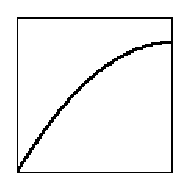
\includegraphics[width=0.20\linewidth]{graphics/Week01_DerivativeDefinition/aableson-4855-setUnit_02_DerivativeDefinitionprob1image6}
 &4. &\includegraphics[width=0.20\linewidth]{graphics/Week01_DerivativeDefinition/aableson-4855-setUnit_02_DerivativeDefinitionprob1image5}
 \\ \hline 
5. &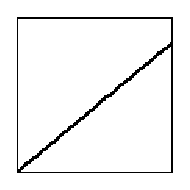
\includegraphics[width=0.20\linewidth]{graphics/Week01_DerivativeDefinition/aableson-4855-setUnit_02_DerivativeDefinitionprob1image1}
 &6. &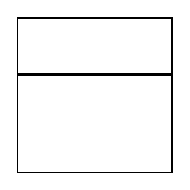
\includegraphics[width=0.20\linewidth]{graphics/Week01_DerivativeDefinition/aableson-4855-setUnit_02_DerivativeDefinitionprob1image2}
 \\ \hline 
 7. &\includegraphics[width=0.20\linewidth]{graphics/Week01_DerivativeDefinition/aableson-4855-setUnit_02_DerivativeDefinitionprob1image3}
 &8. &\includegraphics[width=0.20\linewidth]{graphics/Week01_DerivativeDefinition/aableson-4855-setUnit_02_DerivativeDefinitionprob1image8}
 \\ \hline 
\end {tabular}\end{center}\par\smallskip
\end{center} 
\par 
\par  \end{Question}
\begin{Solution}
 
Because the car is driven at a decreasing speed, the distance 
traveled for different time intervals of the same length must 
decrease as time goes on.  Therefore the slope of the graph 
of distance traveled must decrease with increasing time, and 
must be 3.
\par\end{Solution}
\item
\begin{Question}
 A car is driven at a constant speed, starting at noon.  Which of the following
could be a graph of the distance the car has traveled as a function
of time past noon?
\par 
\begin{center} 
\par\smallskip\begin{center}\begin{tabular}{|c|c|c|c|} \hline
1. &\includegraphics[width=0.20\linewidth]{graphics/Week01_DerivativeDefinition/aableson-2062-setUnit_02_DerivativeDefinitionprob2image4}
 &2. &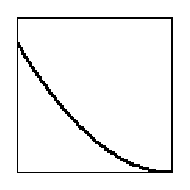
\includegraphics[width=0.20\linewidth]{graphics/Week01_DerivativeDefinition/aableson-2062-setUnit_02_DerivativeDefinitionprob2image7}
 \\ \hline 
 3. &\includegraphics[width=0.20\linewidth]{graphics/Week01_DerivativeDefinition/aableson-2062-setUnit_02_DerivativeDefinitionprob2image6}
 &4. &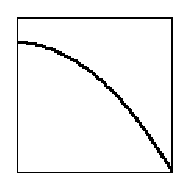
\includegraphics[width=0.20\linewidth]{graphics/Week01_DerivativeDefinition/aableson-2062-setUnit_02_DerivativeDefinitionprob2image5}
 \\ \hline 
5. &\includegraphics[width=0.20\linewidth]{graphics/Week01_DerivativeDefinition/aableson-2062-setUnit_02_DerivativeDefinitionprob2image1}
 &6. &\includegraphics[width=0.20\linewidth]{graphics/Week01_DerivativeDefinition/aableson-2062-setUnit_02_DerivativeDefinitionprob2image2}
 \\ \hline 
 7. &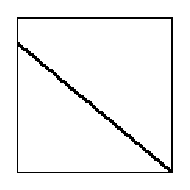
\includegraphics[width=0.20\linewidth]{graphics/Week01_DerivativeDefinition/aableson-2062-setUnit_02_DerivativeDefinitionprob2image3}
 &8. &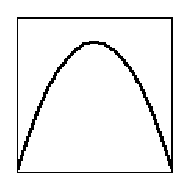
\includegraphics[width=0.20\linewidth]{graphics/Week01_DerivativeDefinition/aableson-2062-setUnit_02_DerivativeDefinitionprob2image8}
 \\ \hline 
\end {tabular}\end{center}\par\smallskip
\end{center} 
\par 
\par  \end{Question}
\begin{Solution}
 
Because the car is driven at a constant speed, the change in the 
distance traveled is the same for different time intervals of the 
same length.  Thus the graph of the distance traveled must have 
a constant positive slope, and must be graph 5.
\par\end{Solution}
\item
\begin{Question}
 Match the points labeled on the curve below with the given slopes in the
following table.
\begin{center} 
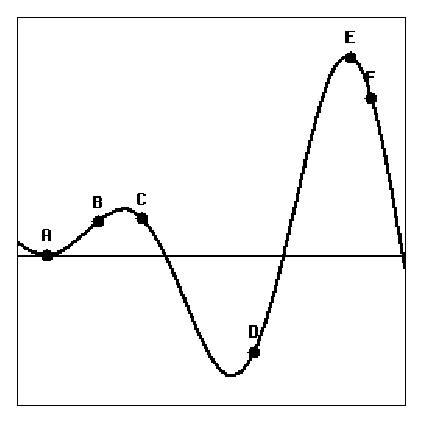
\includegraphics[width=0.5\linewidth]{graphics/Week01_DerivativeDefinition/aableson-4563-setUnit_02_DerivativeDefinitionprob3image1}
\par 
\par\smallskip\begin{center}\begin{tabular}{|c|c|c|c|c|c|c|} \hline
slope &-3 &-1 &-1/2 &0 &1 &2 \\ \hline 
label &&&&&&\\ \hline 
\end {tabular}\end{center}\par\smallskip
\end{center} 
\par  \end{Question}
\begin{Solution}
 
We match the points and slopes by noting that the slope is zero where the
tangent to the curve is horizontal, negative where the function is
decreasing, and positive where the function is increasing.  The magnitude
of the slope gives the rate at which the function is increasing or
decreasing, so that we have
\par 
\par\smallskip\begin{center}\begin{tabular}{|c|c|c|c|c|c|c|} \hline
slope &-3 &-1 &-1/2 &0 &1 &2 \\ \hline 
label &F &C &E &A &B &D \\ \hline 
\end {tabular}\end{center}\par\smallskip
\par\end{Solution}
\item
\begin{Question}
 Consider the function shown in the graph below.
\par 
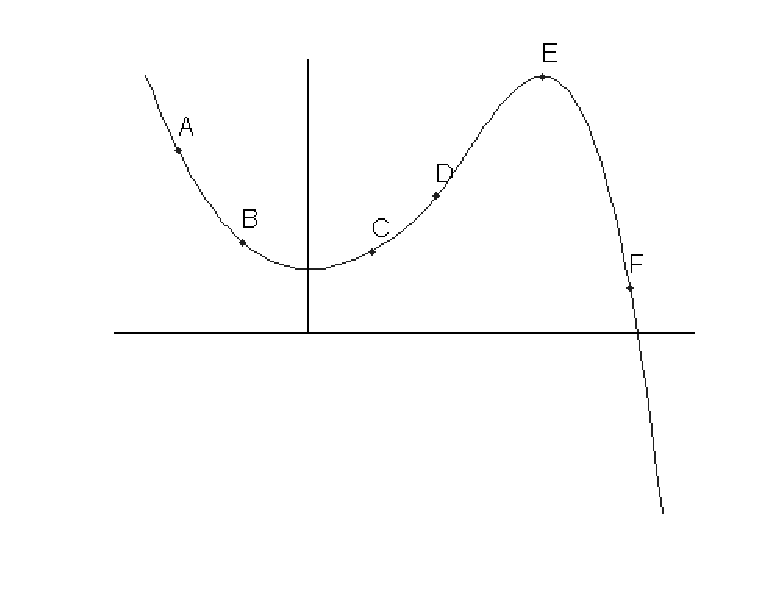
\includegraphics[width=0.7\linewidth]{graphics/Week01_DerivativeDefinition/q_001_3}
\par 
(a)For each labelled point, is the slope of the graph positive, negative or zero?  \\
(b) At which labeled point does the graph have the greatest ( i. e., most positive) slope?  \\
(c) At which labeled point does the graph have the {\bf largest negative} slope?  \\
\par\end{Question}
\begin{Solution}
 {
\vspace{-\parskip}\begin{enumerate}[(a)]
\item ~\begin{enumerate}[A.]
\item Negative 
\item Negative 
\item Positive 
\item Positive 
\item Zero 
\item Negative 
\end{enumerate}
\item D 
\item F 
\end{enumerate}}\par

\end{Solution}
\item
\begin{Question}
 Consider the {\bf  distance vs time } graph shown below.
\par 
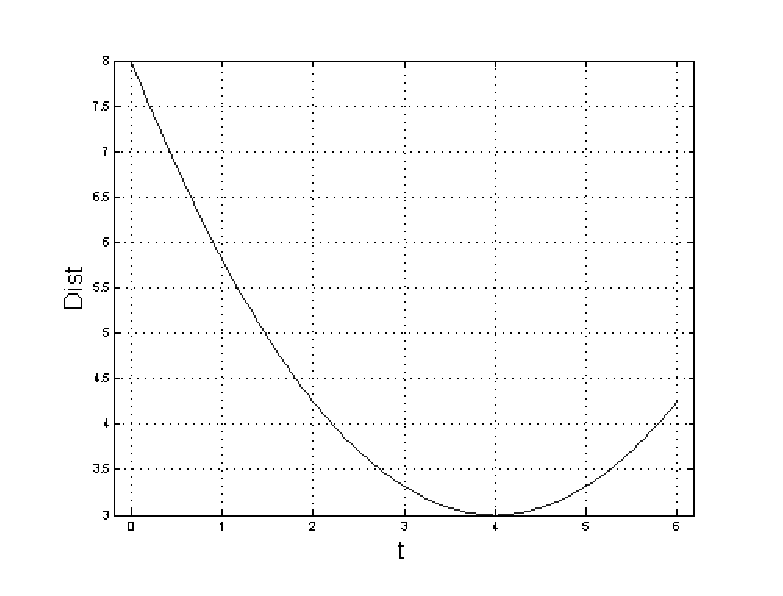
\includegraphics[width=0.7\linewidth]{graphics/Week01_DerivativeDefinition/q_002_4}
\par 
Rank the following quantities as if along the real line (i.e. largest negative, through zero, up to largest positive). \\
A - Instantaneous velocity at \(t=1\). \leavevmode\\\relax 
B - Instantaneous velocity at \(t=3\). \leavevmode\\\relax 
C - Instantaneous velocity at \(t=4\). \leavevmode\\\relax 
D - Instantaneous velocity at \(t=5\). \leavevmode\\\relax 
E - Average velocity over \(t=1 \ldots 3\). \leavevmode\\\relax 
F - Average velocity over \(t=4 \ldots 5\).
\par\end{Question}
\begin{Solution}
\vspace{-\parskip}
The order, from largest negative through to largest positive, is: \\
$A \to E \to B \to C \to F \to D  $

\end{Solution}
\item
\begin{Question}
 
\par 
Let \(f(x)\) be the function whose graph is shown below.
\par 
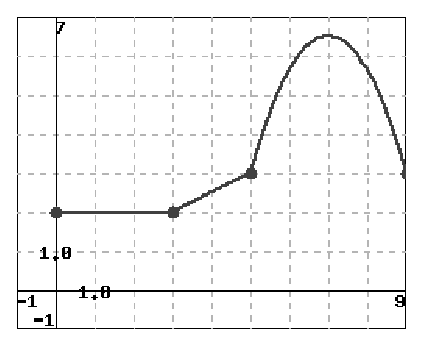
\includegraphics[width=0.8\linewidth]{graphics/Week01_DerivativeDefinition/aableson-4855-setUnit_02_DerivativeDefinitionprob6image1}
\par 
Determine the derivative of \(f(a)\) at the points \(a = 1,2,4,7\).
\par  \end{Question}
\begin{Solution}
 
Remember that the value of the derivative of \(f\) at \(x=a\) can be interpreted as the slope of the line tangent to the graph of \(y = f(x)\) at \(x=a\).  From the figure, we see that the graph of \(y = f(x)\) is a horizontal line (that is, a line with zero slope) on the interval \(0 \le x \le 3\).  Accordingly, \(f'(1) = f'(2) = 0\).  On the interval \(3 \le x \le 5\), the graph of \(y = f(x)\) is a line of slope \(0.5\); thus, \(f'(4) = 0.5\).  Finally, the line tangent to the graph of \(y = f(x)\) at \(x=7\) is horizontal, so \(f'(7) = 0\).
\par\end{Solution}

\item
\begin{Question}
 
\par 
Let \(f(x)\) be the function whose graph is shown below.
\par 
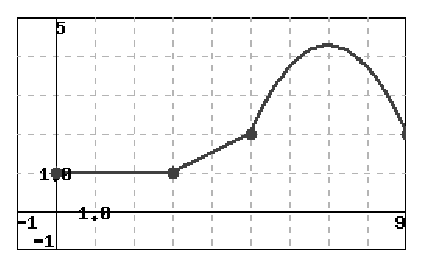
\includegraphics[width=0.8\linewidth]{graphics/Week01_DerivativeDefinition/aableson-2062-setUnit_02_DerivativeDefinitionprob7image1}
\par 
Which is larger?
\begin{itemize}
\item{A. \(f'(6.5)\)}
\item{B. \(f'(5.5)\)}
\end{itemize}
\par  \end{Question}
\begin{Solution}
 
The line tangent to the graph of \(y = f(x)\) at \(x = 5.5\) has a larger slope than the line tangent to the graph of \(y = f(x)\) at \(x = 6.5\).  Therefore, \(f'(5.5)\) is larger than \(f'(6.5)\).
\par\end{Solution}
\item
\begin{Question}
 Use algebra to evaluate the following limit.
\par 
\(\ds \lim\limits_{h \rightarrow 0} \frac{(3+h)^2- 9  }{h} \)
\par  \end{Question}
\begin{Solution}
 
\(\frac{(3+h)^2- 9}{h} =
     \frac{3^2+6 h + h^2- 9}{h} =
	\frac{6 h + h^2}{h}=6+h\)
\par 
Thus, as \(h\to 0\) we have
\(\frac{(3+h)^2- 9}{h} \to 6\).
\par\end{Solution}
\item
\begin{Question}
 Estimate the following limit by substituting smaller and smaller values of
\(h\), and by using algebra (the two answers should be very similar!).
\par 
\(\ds \lim \limits_{h \rightarrow 0} \frac{(4+h)^3- 64  }{h} \)
\par  \end{Question}
\begin{Solution}
 
We try successively smaller values of \(h\):
\(\frac{(4+0.1)^3-64}{0.1}=49.2100\)
\(\frac{(4+0.01)^3-64}{0.01}=48.1201\)
\(\frac{(4+0.001)^3-64}{0.001}=48.0120\)
\(\frac{(4+0.0001)^3-64}{0.0001}=48.0012\)
\(\frac{(4+0.00001)^3-64}{0.00001}=48.0001\)
\par 
These values suggest that the limit is 48.000.
\par\end{Solution}
\item
\begin{Question}
 Suppose \(y = f(x)\) graphed in the figure below
represents the cost of manufacturing \(x\) kilograms of a chemical.
\par 
\begin{center} 
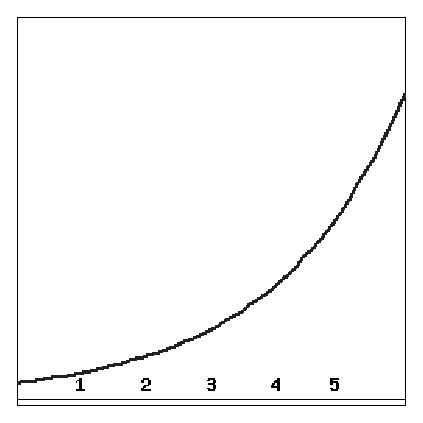
\includegraphics[width=0.5\linewidth]{graphics/Week01_DerivativeAtAPoint/aableson-2134-setUnit_02_DerivativeAtAPointprob1image1}
\end{center} 
\par 
\(f(x)/x\) represents the average cost of
producing 1 kilogram of the chemical when \(x\) kilograms are made.
This problem asks you to visualize these averages graphically.
\par 
\begin{enumerate}[(a)]
\item We can represent \(f(4)/4\) as the slope of a line.  Through what
points does this line extend?
\item Which is larger, \(f(3)/3\) or \(f(4)/4\)?
\end{enumerate}
\par  \end{Question}
\begin{Solution}
\begin{enumerate}[(a)] 
\item \(f(4)/4\) is the slope of the line connecting
\((0,0)\) to \((4,f(4))\), as shown below.
\par 
\begin{center} 
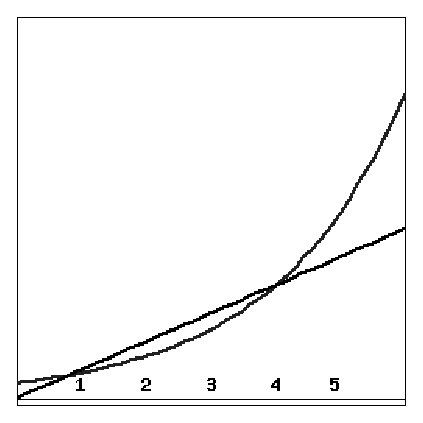
\includegraphics[width=0.5\linewidth]{graphics/Week01_DerivativeAtAPoint/aableson-2134-setUnit_02_DerivativeAtAPointprob1image2}
\end{center} 
\par 
\item Extending the line described in part (a) for both the points $x=3$ and $x=4$, we will get a higher slope in the second case, so 
\[\ds \frac{f(3)}{3} < \frac{f(4)}{4}\]
\end{enumerate}
\par\end{Solution}
\item
\begin{Question}
 Consider the function \(y = f(x)\) graphed below.
\par 
\begin{center} 
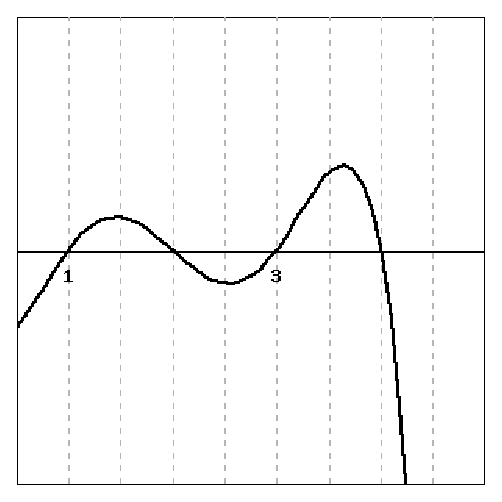
\includegraphics[width=0.5\linewidth]{graphics/Week01_DerivativeAtAPoint/aableson-1303-setUnit_02_DerivativeAtAPointprob2image1}
\end{center} 
\par 
Give the \(x\)-coordinate of a point where:
\begin{enumerate}[(a)]
\item The derivative of the function is positive.
\item The value of the function is positive.
\item The derivative of the function is largest.
\item The derivative of the function is zero.
\item The derivative of the function is approximately the same
as the derivative at \(x = 3.25\).
\end{enumerate}
\par  \end{Question}
\begin{Solution}
\begin{enumerate}[(a)] 
\item Recall that the derivative is positive when the function is increasing.  So
we're looking for a point on the graph where the function is increasing;
one such point is \(x = 1\).
\par 
\item
The function is positive when the function is above the \(x\)-axis.  One such point is
\(x = 1.5\).
\par 
\item
The derivative of the function is largest when the function is increasing
the fastest. This occurs at \(x \approx 3.25\).
\par 
\item
The derivative of the function is zero when the function has a horizontal
tangent.  One such point is \(x \approx 1.45\).
\par 
\item
Finally, we're looking for a point where the derivative is the same as the
derivative at \(x = 3.25\).  This means that we want the slope of a tangent
to the curve to be approximately the same as it is at \(x = 3.25\).  Such a
point is \(x = 0.75\).
\end{enumerate}
\par\end{Solution}
\item
\begin{Question}
 Consider the graph of the function \(f(x)\) shown below.
\par 
\begin{center} 
\includegraphics[width=0.5\linewidth]{graphics/Week01_DerivativeAtAPoint/aableson-2475-setUnit_02_DerivativeAtAPointprob3image1}
\end{center} 
\par 
Using this graph, for each of the following pairs of numbers
decide which is larger.  {\it Be sure that you can explain your
answer.} 
\par 
\begin{enumerate}[(a)]
\item
\(f(8)\) vs. \(f(10)\)
\item
\(f(8) - f(6)\) vs. \(f(6) - f(4)\)
\item
\(\ds \frac{f(6) - f(4)}{6 - 4}\)
  vs.
  \(\ds \frac{f(8) - f(4)}{8 - 4}\)
\item
\(f'(4)\) vs. \(f'(10)\)
\end{enumerate}
\par  \end{Question}
\begin{Solution}
\begin{enumerate}[(a)] 
\item
Since \(f\) is increasing,
\(f(8) < f(10)\).
\item
From the figure, it appears that
\(f(8) - f(6) > f(6) - f(4)\).
\item
The quantity \(\frac{f(6)-f(4)}{6-4}\)
represents the slope of the secant line connecting the points on the graph
at \(x=4\) and \(x=6\). This is less than the slope of the
secant line connecting the points at \(x=4\) and \(x=8\), which
is \(\frac{f(8)-f(4)}{8-4}\)
\item
The function is less steep at \(x=4\) than at \(x=10\), so
\(f'(4) < f'(10)\).
\end{enumerate}
\par\end{Solution}
\end{multicols}



\hrulefill
\subsection*{The Derivative as a Function}

\begin{multicols}{2}
\item
\begin{Question}
 Consider the function \(f(x)\) shown in the graph below.
\begin{center} 
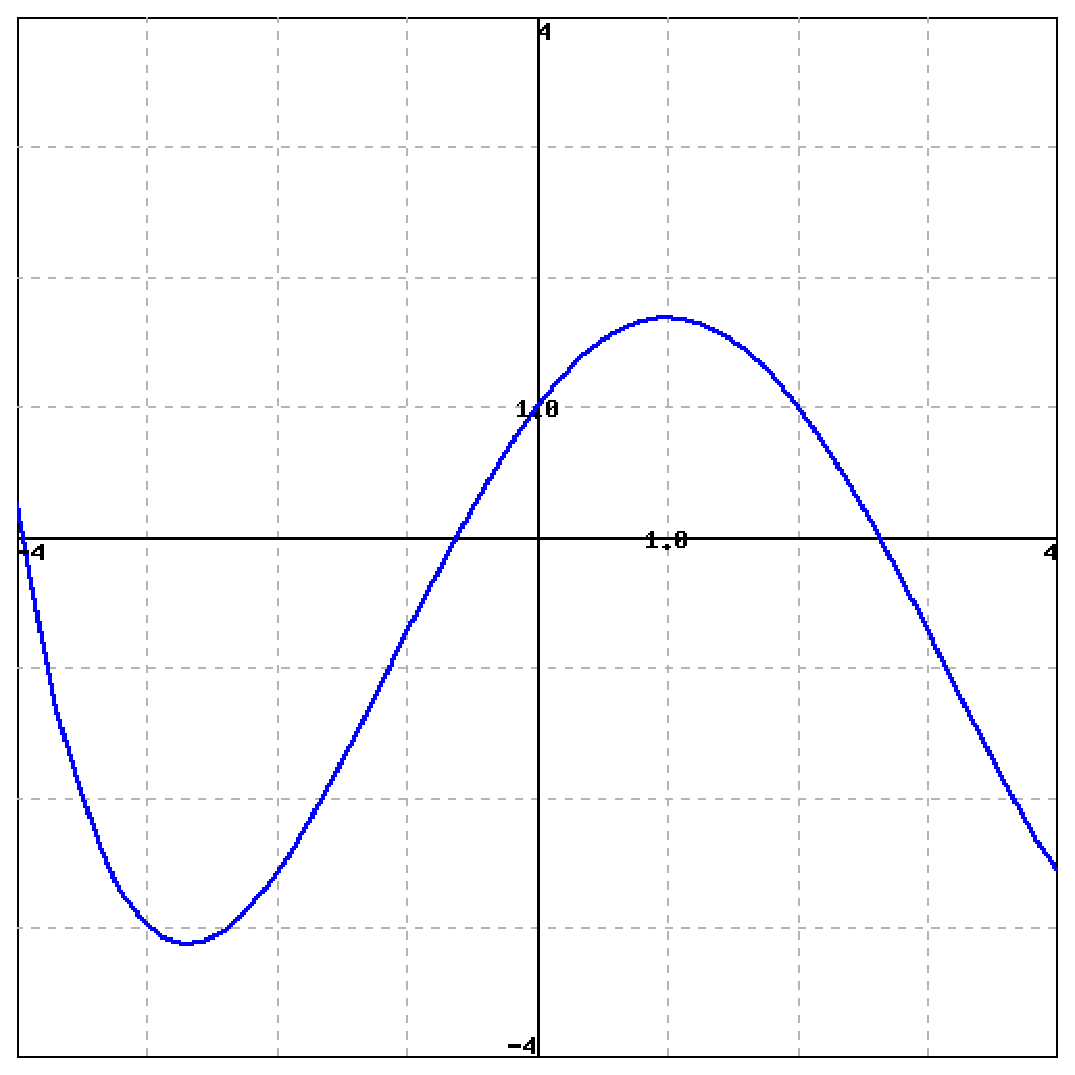
\includegraphics[width=0.5\linewidth]{graphics/Week01_DerivativeFunction/aableson-1955-setUnit_03_DerivativeFunctionprob2image1}
\end{center} 
\par 
Carefully sketch the derivative of the given function (you will want
to estimate values on the derivative function at different \(x\)
values as you do this).  Use your derivative function graph to
estimate the following values on the derivative function.
\par 
\begin{center} 
\par\smallskip\begin{center}\begin{tabular}{|c|c|c|c|c|} \hline
at \(x =\) &-3 &-1 &1 &3 \\ \hline 
the derivative is &\mbox{\parbox[t]{3ex}{\hrulefill}} &\mbox{\parbox[t]{3ex}{\hrulefill}} &\mbox{\parbox[t]{3ex}{\hrulefill}} &\mbox{\parbox[t]{3ex}{\hrulefill}} \\ \hline 
\end {tabular}\end{center}\par\smallskip
\end{center} 
\par  \end{Question}
\begin{Solution}
 
At each value of \(x\), we estimate the derivative by estimating the 
slope (=rise/run) from the graph.  This allows us to both sketch the
graph of the derivative and estimate the derivatives that are requested.
The derivative (in red) is shown with the original function (in blue)
below.
\par 
\begin{center} 
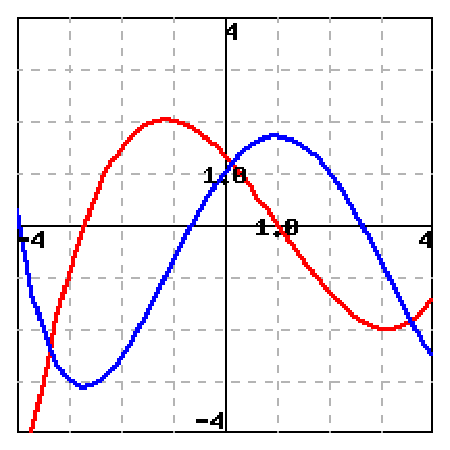
\includegraphics[width=0.5\linewidth]{graphics/Week01_DerivativeFunction/aableson-1955-setUnit_03_DerivativeFunctionprob2image2}
\end{center} 
\par 
From the graph and our calculations, it appears that
\(f'(-3) \approx -1\), \leavevmode\\\relax 
\(f'(-1) \approx 2\), \leavevmode\\\relax 
\(f'(1) \approx 0\), and \leavevmode\\\relax 
\(f'(3) \approx -2\). \leavevmode\\\relax 
\par\end{Solution}
\item
\begin{Question}
Below is the graph of \(f(x)\). Sketch the graph of $f'(x)$.
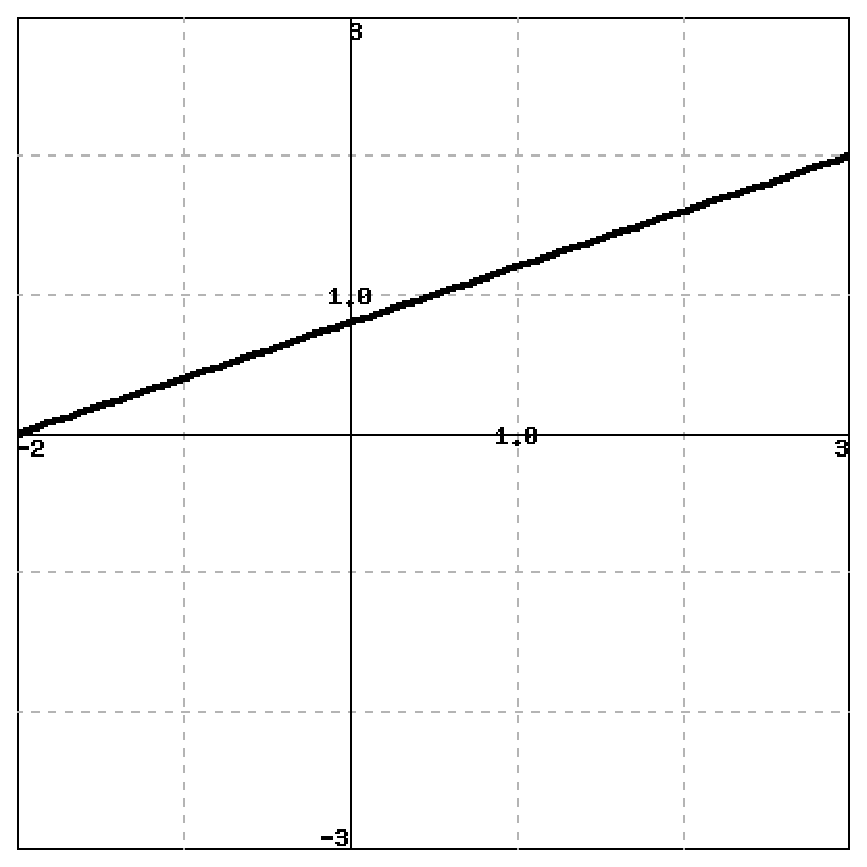
\includegraphics[width=0.3\linewidth]{graphics/Week01_DerivativeFunction/aableson-4521-setUnit_03_DerivativeFunctionprob5image1}
\par 
\par\end{Question}
\begin{Solution}
 
The {\bf slope} on the original function is constant, so the {\bf derivative} value is constant.

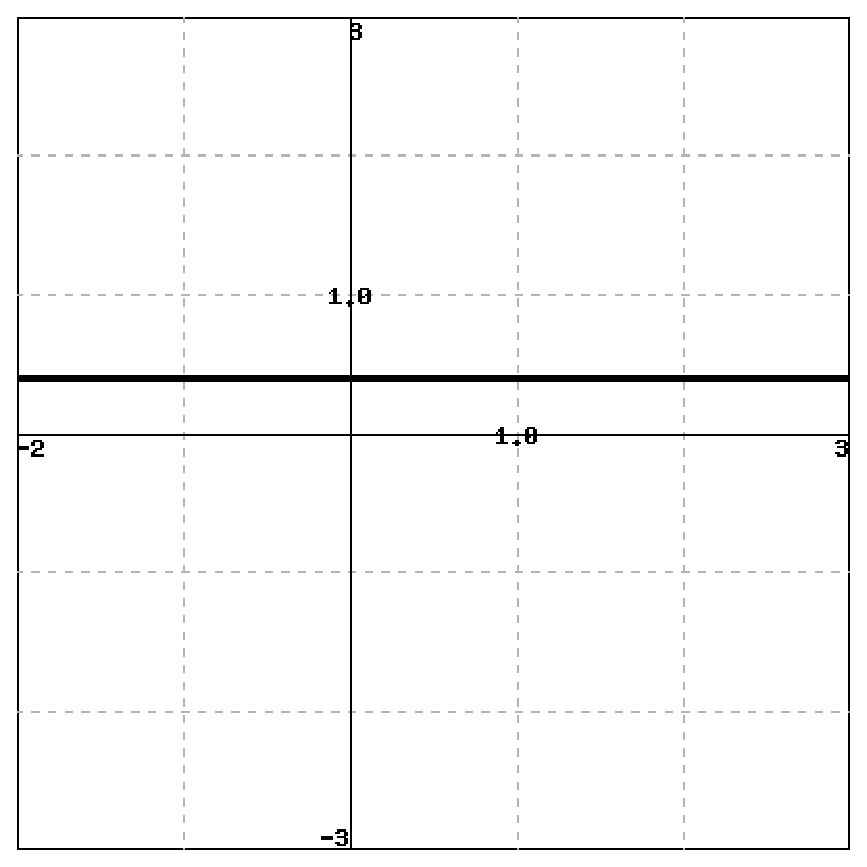
\includegraphics[width=0.3\linewidth]{graphics/Week01_DerivativeFunction/aableson-4521-setUnit_03_DerivativeFunctionprob5image2}

\end{Solution}
\item
\begin{Question}
Below is the graph of \(f(x)\). Sketch the graph of $f'(x)$.
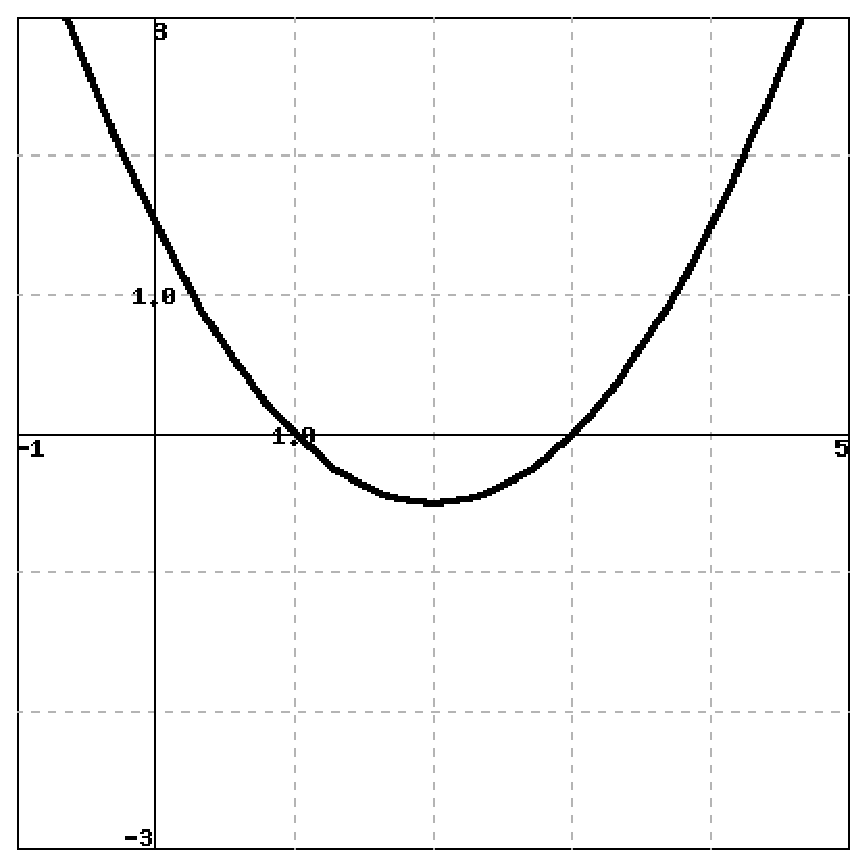
\includegraphics[width=0.5\linewidth]{graphics/Week01_DerivativeFunction/aableson-1624-setUnit_03_DerivativeFunctionprob6image1}
\par 
\par\end{Question}
\begin{Solution}
There is a point with {\bf slope} zero at $x=2$, so there must be a {\bf derivative} value of zero at $x=2$. \\
For smaller values of $x$, the {\bf slopes} are negative, so the {\bf derivative} values will be negative. \\
For larger values of $x$, the {\bf slopes} are positive, so the {\bf derivative} values will be positive. \\

\hfil 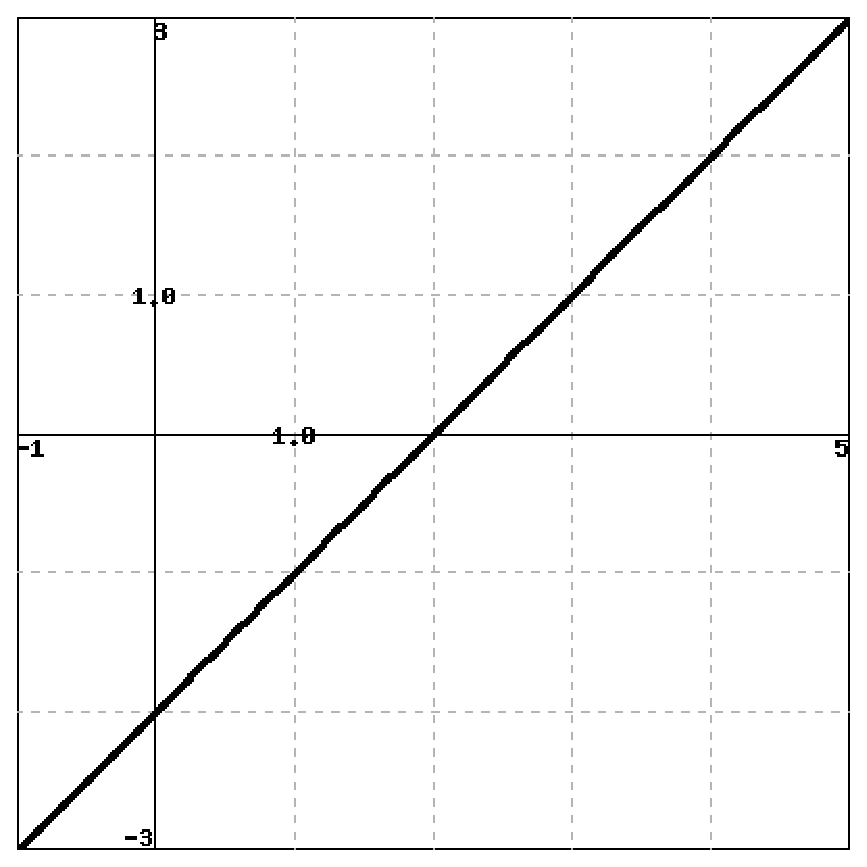
\includegraphics[width=0.50\linewidth]{graphics/Week01_DerivativeFunction/aableson-1624-setUnit_03_DerivativeFunctionprob6image2}

Note that the graph of $f'(x)$ shown here has an accurate vertical
scale; however, that would be difficult for you to estimate by eye
based simply on the graph of $f(x)$, so we do not expect that level of
precision on a test or exam.

\end{Solution}
\item
\begin{Question}
Below is the graph of \(f(x)\). Sketch the graph of $f'(x)$.
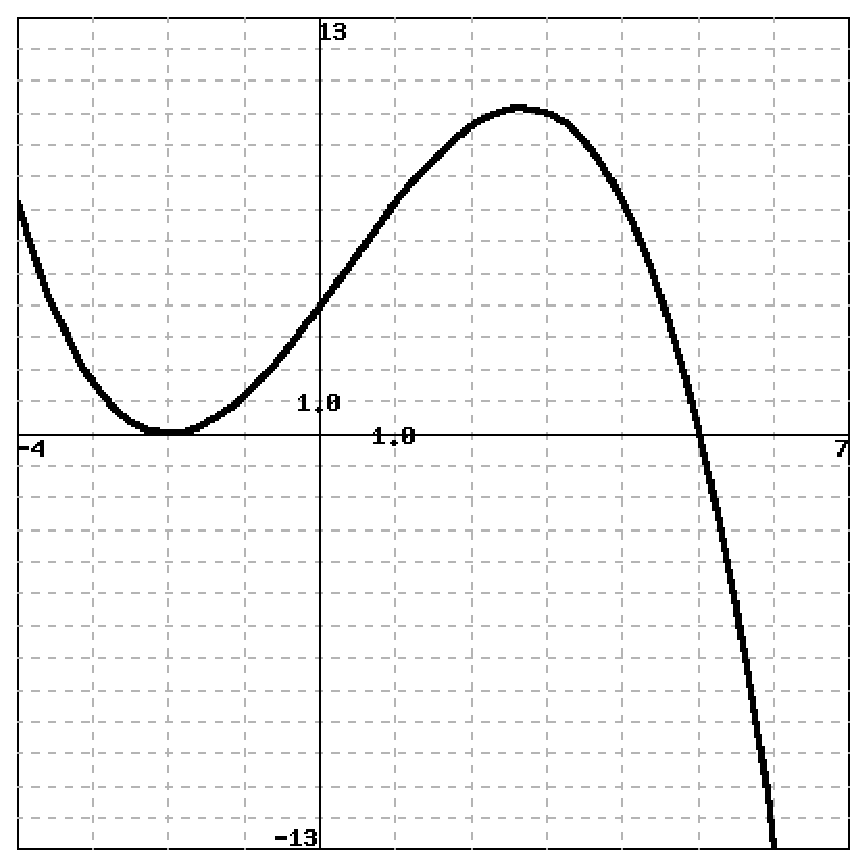
\includegraphics[width=0.6\linewidth]{graphics/Week01_DerivativeFunction/aableson-880-setUnit_03_DerivativeFunctionprob7image1}
\par\end{Question}
\begin{Solution}
There are two points with {\bf slope} zero, at $x=2$ and $x \approx 2.5$, so there must be a {\bf derivative} value of zero at those two $x$ locations. \\
In between those landmark points, the slopes of $f$ go: negative, positive, negative.

 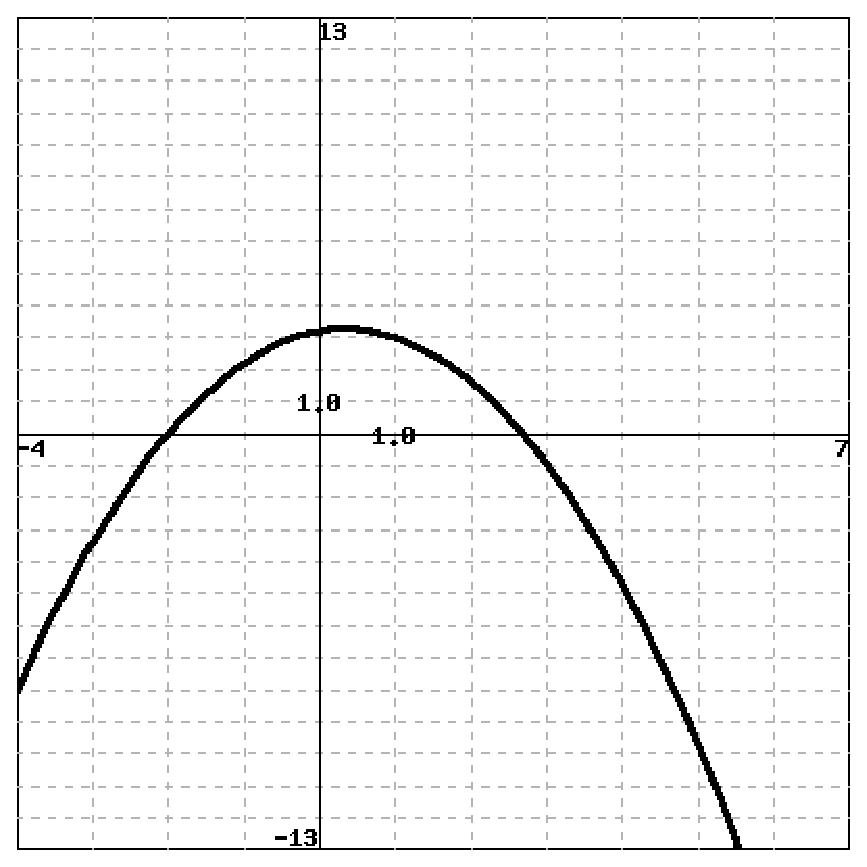
\includegraphics[width=0.60\linewidth]{graphics/Week01_DerivativeFunction/aableson-880-setUnit_03_DerivativeFunctionprob7image2}

Note that the graph of $f'(x)$ shown here has an accurate vertical
scale; however, that would be difficult for you to estimate by eye
based simply on the graph of $f(x)$, so we do not expect that level of
precision on a test or exam.

\end{Solution}
\item \begin{Question}
  For the function \(f(x)\) shown in the graph below, sketch a graph
  of the derivative.
\par 
\begin{center} 
\includegraphics[width=0.6\linewidth]{graphics/Week01_DerivativeFunction/aableson-4073-setUnit_03_DerivativeFunctionprob3image1}
\end{center} 
\par 
\par  \end{Question}
\begin{Solution}
 
Because the derivative gives the slope of the original function at
each point \(x\), we know that the derivative is negative where
\(f(x)\) is decreasing and positive where it is increasing.  Applying
this to \(f(x)\), a sketch of the derivative would resemble the graph below:
\par 
\begin{center} 
\includegraphics[width=0.5\linewidth]{graphics/Week01_DerivativeFunction/aableson-4073-setUnit_03_DerivativeFunctionprob3image2}
\end{center} 
\par\end{Solution}
\item 
\begin{Question}
 A child fills a pail by using a water hose.  After finishing, the child
plays in a sandbox for a while before tipping the pail over to empty it.  
If \(V(t)\) gives the volume of the water in the pail at time \(t\),
then the figure below shows \(V'(t)\) as a function of \(t\).
\par 
\begin{center} 
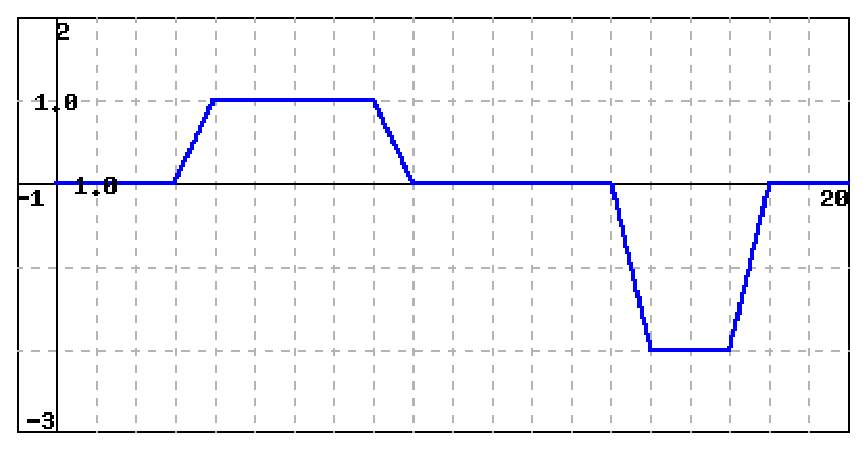
\includegraphics[width=0.5\linewidth]{graphics/Week01_DerivativeFunction/aableson-3218-setUnit_03_DerivativeFunctionprob4image1}
\end{center} 
\par 
At what time does the child:
\begin{enumerate}[(a)]
\item Begin to fill the pail?
\item Finish filling the pail?
\item Tip the pail over?
\end{enumerate}
\par  \end{Question}
\begin{Solution}
 
The child begins filling the pail when \(V'(t)\) becomes positive,
which is when the volume of water in the pail starts increasing.  This is
at \(t = 3\).  The child finishes filling the pail when the volume stops
increasing, which is at \(t = 9\).  The child tips the pail over when the 
volume of water in the pail start decreasing, which is where  \(V'(t)\)
first becomes negative, which is at \(t=14\).
\par\end{Solution}
\end{multicols}

\hrulefill

\subsection*{Computing Derivatives}

Below are a {\bf small sample of problems} involving the computation
of derivatives.  They are {\bf not enough} to properly learn and
memorize how to apply all the derivative rules.  You should practice
with as many problems as you need to become proficient at computing
derivatives.

Further practice problems can be found in any calculus textbook.    For example,

\begin{multicols}{2}

From Hughes-Hallett 5th edition,  \\
Section 3.1 - 7-47 (odd)\symbolfootnote[2]{For this section, simplify products and fractions {\em before} you differentiate, rather than using the product rule and quotient rule.} \\
Section 3.2 - 1-33 (odd)  \\
Section 3.3 - 3-29 (odd) \\
Section 3.4 - 1-49 (odd) \\
Section 3.5 - 3-39 (odd) \\  % All pure differentiation problems; no word problems
Section 3.6 - 1-33 (odd)

\columnbreak

From Hughes-Hallett 6th edition,  \\
Section 3.1 - 7-49 (odd)\symbolfootnote[2]{For this section, simplify products and fractions {\em before} you differentiate, rather than using the product rule and quotient rule.} \\
Section 3.2 - 1-25 (odd)  \\
Section 3.3 - 3-29 (odd) \\
Section 3.4 - 1-55 (odd) \\
Section 3.5 - 3-47 (odd) \\  % All pure differentiation problems; no word problems
Section 3.6 - 1-41 (odd)

\end{multicols}

\hrulefill

\begin{multicols}{2}
\item
\begin{Question}
 Let \(f(x) =  4 e^x - 9 x^2 + 5\). Compute  \(f'( x )\).
\par\end{Question}
\begin{Solution}
$f'(x) = 4e^x - 18 x$

\end{Solution}
\item
\begin{Question}
\par 
Let \(\displaystyle f(x) =  2 x^{6} \sqrt{x} + \frac{-5} {x^{3} \sqrt{x} }\). Compute $f'(x)$.
\par 
\par\end{Question}
\begin{Solution}
You can use the product rule here if you like, but it is far easier to rewrite the function before you start, 
since all the terms are just powers of $x$.
\begin{align*}
f(x) & =  2 x^{6} \sqrt{x} + \frac{-5} {x^{3} \sqrt{x}}  \\
f(x) & =  2 x^{6} \cdot x^{1/2} + \frac{-5} {x^{3} \cdot x^{1/2}}  \\
& = 2 x^{\frac{13}{2}} -5 x^{\frac{-7}{2}}
\end{align*}
Differentiating,
\begin{align*}
f'(x) & = 2 \frac{13}{2}x^{\frac{11}{2}} -5\left(\frac{-7}{2}\right) x^{\frac{-9}{2}} \\
& = 13 x^5 \sqrt{x} + \frac{35}{2 x^4 \sqrt{x}}
\end{align*}

\end{Solution}
\item
\begin{Question}
 Let 
\(\ds f(x) =  \frac { 7 x^2 + 7 x + 5 } {\sqrt{x} }\).

(a) Compute \(f'( x )\).  \hfill (b) Find \(f'( 3 )\).\hfill \hfill 
\par\end{Question}
\begin{Solution}
You can use the quotient rule here if you like, but it is far easier to rewrite the function before you start, 
since all the terms are just powers of $x$.
\begin{align*}
f(x)&  =  \frac { 7 x^2 + 7 x + 5 } {\sqrt{x} } \\
& = 7 x^{3/2} + 7 x^{1/2} + 5 x^{-1/2}
\end{align*}
\begin{enumerate}[(a)]
\item $\ds f'(x) = \frac{21}{2} x^{1/2} + \frac{7}{2} x^{-1/2} - \frac{5}{2} x^{-3/2}$
\item Evaluating $f'(x)$ at $x=3$, we obtain $\approx 19.726$.
\end{enumerate}

\end{Solution}
\item
\begin{Question}
 Let \(f(t) =  7 t^{-7}\). 

(a) Compute \(f'( t )\). \hfill (b) Find \(f'( 3 )\). \hfill \hfill
\par\end{Question}
\begin{Solution}
\begin{enumerate}[(a)]
\item $f'(x) = -49 ~t^{-8}$
\item $f'(3) = -49 ~(3^{-8})$
\end{enumerate}

\end{Solution}
\item
\begin{Question}
 Let \(f(x) =  4 e^{x} + e^{1}\). Compute \(f'( x ) .\) 
\par\end{Question}
\begin{Solution}
Don't be thrown off by the $e^{1}$: that's a constant (equal to $e$ or $\approx$ 2.7), so the derivative of that term is zero. 

$f'(x) = 4 e^{x}$ 

\end{Solution}
\item
\begin{Question}
 Let \(f(x) =  4 e^{x} + 4 x\). Compute \(f'( x ).\)
\par\end{Question}
\begin{Solution}
$f'(x) = 4 e^x +4$
\end{Solution}
\item
\begin{Question}
 \(f(x) =  (3 x^2 - 2 )(6 x + 3)\). 

(a) Compute \(f'( x )\). \hfill
(b) Find \(f'( 4 )\). \hfill \hfill
\par\end{Question}
\begin{Solution}
You can either expand the product before differentiating (and obtain $f(x) = 18x^3 +9x^2-12x-6$), or use the product rule.  Both give the same answer.
\begin{enumerate}[(a)]
\item $f'(x) =  54x^2 + 18x -12$.
\item $f'(4) = 924$.
\end{enumerate}

\end{Solution}
\item
\begin{Question}
\par 

Let \(\ds f(x) =  \frac {\sqrt { x } - 4 } {\sqrt { x } + 4 }\).  Compute $f'(9)$.
\par\end{Question}
\begin{Solution}
We need to use the quotient rule for this function.
\begin{align*}
f'(x) & = \frac{\frac{1}{2}x^{-1/2}(x^{1/2} + 4) - (x^{1/2}-4)\left(\frac{1}{2}\right)x^{-1/2}}{ (\sqrt{x} + 4)^2} \\
& = \frac{1 + 4/\sqrt{x} - 1 + 4/\sqrt{x}}{2(\sqrt{x} + 4)^2} \\ 
& = \frac{4}{\sqrt{x} (\sqrt{x} + 4)^2} \\ 
f'(9) & = \frac{4}{3 (3 + 4)^2} \\ 
& = \frac{4}{147}
\end{align*}

\end{Solution}
\item
\begin{Question}
 Consider $\ds f(x) =  \frac { 4 x +  3 } { 3 x + 2 }$.

(a) Compute \(f'( x )\). \hfill
(b) Find \(f'( 5 )\). \hfill \hfill
\par\end{Question}
\begin{Solution}
\begin{enumerate}[(a)]
\item $\ds f'(x) = \frac{4(3x+2) - (4x+3)(3)}{(3x+2)^2}$
\item $\ds f'(5) = \frac{-1}{17^2}$ 
\end{enumerate}

\end{Solution}
\item
\begin{Question}
Consider $\ds f(x) =  \frac { 7 - x^2 } { 7 + x^2 }$

(a) Compute \(f'( x )\). \hfill
(b) Find \(f'( 1 )\). \hfill \hfill
\par\end{Question}
\begin{Solution}
\begin{enumerate}[(a)]
\item $\ds f'(x) = \frac{-28x}{ (x^2 + 7)^2}  $
\item $\ds f'(1) = \frac{-28}{ 64}  $
\end{enumerate}

\end{Solution}
\item
\begin{Question}
Let \(f(x) = -2 x(x-3)\).

(a) Compute \(f'(x)\). \hfill (b) Find \(f'(-5)\). \hfill \hfill
\par\end{Question}
\begin{Solution}
\begin{enumerate}[(a)]
\item $f'(x) = -4x+6$
\item $f'(-5) = 26$
\end{enumerate}
\end{Solution}
\item
\begin{Question}
$\ds f(x) =  \frac {4 x^3- 3} {x^4}$

(a) Compute \(f'( x )\). \hfill
(b) Find \(f'( 2 )\). \hfill \hfill
\par\end{Question}
\begin{Solution}
\begin{enumerate}[(a)]
\item $-4x^{-2}+12x^{-5}$
\item $-0.625$
\end{enumerate}

\end{Solution}
\item
\begin{Question}
$\ds g(x) = \frac{e^x}{5 + 4x}$.  Compute $g'(x)$.
\par\end{Question}
\begin{Solution}
$\ds g'(x) = \frac{(1 +4x )e^x }{(5+4x)^2}$

\end{Solution}
%\item
%\begin{Question}
%$\ds f(x) =  \frac {\sqrt { x } - 5 }{\sqrt { x } + 5 }$
%
%(a) Compute \(f'( x )\). \hfill
%(b) Find \(f'( 2 )\). \hfill \hfill
%\par\end{Question}
%\begin{Solution}
%\begin{enumerate}[(a)]
%\item $\ds f'(x) = \frac{5}{\sqrt{x} (\sqrt{x} + 5)^2}$
%\item $\ds f'(2) = \frac{5}{\sqrt{2} (\sqrt{2} + 5)^2} \approx 0.08593$
%\end{enumerate}
%\end{Solution}
\item
\begin{Question}
\(\ds f(x) =  \frac { 4 x^2 \tan x }{ \sec x }\). 

(a) Find \(f'( x )\).  \hfill
(b) Find \(f'( 3 )\). \hfill \hfill
\par\end{Question}
\begin{Solution}
This should definitely be simplified before you differentiate!  

Recall: $\ds \tan(x) = \frac{\sin(x)}{\cos(x)}$, and $\ds \sec(x) = \frac{1}{\cos(x)}$, 
so $\ds \frac{\tan(x)}{\sec(x)} = \frac{\sin(x)}{\cos(x)} \cos(x) = \sin(x)$.

\begin{enumerate}[(a)]
\item $f'(x) = 8x \sin(x) + 4x^2 \cos(x)$
\item $f'(3) = 24 \sin(3) + 36 \cos(3) \approx -32.253$ 
\end{enumerate}
\end{Solution}
\item
\begin{Question}
\(f(x) = 7 \sin x + 12 \cos x\)

(a)Compute \(f'(x)\). \hfill
(b) Find \(f'( 1 )\). \hfill \hfill
\par\end{Question}
\begin{Solution}

\begin{enumerate}[(a)]
\item $f'(x) = 7\cos(x) - 12 \sin(x)$
\item $f'(1) = 7 \cos(1) - 12 \sin(1) \approx -6.3155$
\end{enumerate}

\end{Solution}
\item
\begin{Question}
Let \(f(x) =  \cos x - 2 \tan x\). Compute \(f'(x)\).
\par\end{Question}
\begin{Solution}
$f'(x) = -\sin(x)-2 \sec^2(x)$
\end{Solution}
\item
\begin{Question}
$\ds f(x) = \frac { 5 \sin x }{ 3 + \cos x }$

(a) Compute \(f'( x )\). \hfill 
(b) Find \(f'( 2 )\).\hfill \hfill
\par\end{Question}
\begin{Solution}
Don't forget the identity $\sin^2(x) + \cos^2(x) = 1$.
\begin{enumerate}[(a)]
\item $f'(x) = (15 \cos(x)+5)/(3+\cos(x))^2$
\item $f'(2) = (15 \cos(2) + 5)/(3 + \cos(2))^2 \approx -0.18606$
\end{enumerate}
\end{Solution}
\item
\begin{Question}
$\ds f(x) = 7 x( \sin x + \cos x) $

(a) Compute $f'(x)$. \hfill
(a) Find $f'(3)$. \hfill \hfill
\par 
\par\end{Question}
\begin{Solution}
\begin{enumerate}[(a)]
\item $f'(x) = 7(\sin(x)+\cos(x))+ 7x(\cos(x)-\sin(x))$
\item $f'(3) \approx -29.695$
\end{enumerate}

\end{Solution}
%\item
%\begin{Question}
% Let \[f(x) = 6 \sin (\sin x)\]
%\par 
%\(f'( x ) =\) \mbox{\parbox[t]{15ex}{\hrulefill}}
%\par\end{Question}
%\begin{Solution}
%\item $6*cos(sin(x))*cos(x)$
%
%\end{Solution}
\item
\begin{Question}
Let  \(\ds f(x) = \cos ( \sin ( x ^2 ))\). Compute $f'(x)$.
\par\end{Question}
\begin{Solution}
$f'(x) = -\sin(\sin(x^2)) \cos(x^2)\cdot (2x)$

\end{Solution}
%\item
%\begin{Question}
% Let \[f(x) = (x^3+ 4 x + 3) ^ { 2 }\]
%\par 
%\(f'( x ) =\) \mbox{\parbox[t]{20ex}{\hrulefill}}
%\par 
%\par\end{Question}
%\begin{Solution}
%$(2*(x**3+4*x+3)**(2-1))*(3*x*x+4)$
%
%\end{Solution}
%\item
%\begin{Question}
% Let \(f(x) = 7 e^{x \cos x}\). \leavevmode\\\relax 
%\(f'( x ) =\) \mbox{\parbox[t]{15ex}{\hrulefill}}
%\par\end{Question}
%\begin{Solution}
%$7*e^(x*cos(x))*(cos(x) - x*sin(x))$
%
%\end{Solution}
\item
\begin{Question}
 Let \(f(x) = 2 \sin ^{3} x\). Compute $f'(x)$. 
\par\end{Question}
\begin{Solution}
$f'(x) = 6\sin^2(x) \cos(x)$

\end{Solution}
\item
\begin{Question}
 Let $y = (8 + \cos^2{x})^{6}$.  Compute $\ds \frac{dy}{dx}$. 
\par 
\par\end{Question}
\begin{Solution}
$\ds \frac{dy}{dx} = 6 (8+cos^2(x))^5(2 \cos(x) (-\sin(x)))$

\end{Solution}
\item
\begin{Question}
 Let $f(x) = -3 \ln[\sin(x)]$.  Compute $f'(x)$.
\par\end{Question}
\begin{Solution}
$\ds f'(x) = \frac{-3}{\sin(x)} \cos(x) \mbox{ or, using trig identities } = -3 \cot(x)$

\end{Solution}
 \item
 \begin{Question}
  Let \(f(x) = 2 \ln(4+x)\). Compute \(f'( x )\).
 \par\end{Question}
 \begin{Solution}
 $\ds f'(x) = \frac{2}{4+x}$
 \end{Solution}
%\item
%\begin{Question}
% If \(f(x) = 2 \cos(5\ln(x))\), find \(f'( x )\).
%Find \(f'( 2 )\).
%\par\end{Question}
%\begin{Solution}
%\item $-2*sin(5*ln(x))*5/x$
%\item 1.59248384128973 
%
%\end{Solution}
%\item
%\begin{Question}
% Let \[f(x) = \ln (x^ {2})\]
%\par 
%\(f'( x ) =\) \mbox{\parbox[t]{20ex}{\hrulefill}}
%\par 
%\(f'( e^{4} ) =\) \mbox{\parbox[t]{20ex}{\hrulefill}}
%\par\end{Question}
%\begin{Solution}
%\item 2 / x 
%\item 0.0366312778022126 
%
%\end{Solution}
%\item
%\begin{Question}
% Let \[f(x) = 9^x \log_{4} (x)\]
%\par 
%\(f'( x ) =\) \mbox{\parbox[t]{20ex}{\hrulefill}}
%\par\end{Question}
%\begin{Solution}
%\item $9^x*(ln(9)*ln(x)/ln(4)+1/x/ln(4))$
%
%\end{Solution}


\item
\begin{Question}
Consider the function $\cos(\arccos(x))$. 
\begin{enumerate}[(a)]
\item Simplify the expression to get a simple equation.
\item Differentiate both sides of the equation, and then solve for
  $\ds \ddx{} \arccos(x)$.
\item Use the trig identity $\sin(\theta) = \sqrt{1 - \cos^2(\theta)}$
    to simplify your expression for $\ds \ddx \arccos(x)$.
\end{enumerate}
\end{Question}

\begin{Solution}
\begin{enumerate}[(a)]
\item Since $\cos$ and $\arccos$ are inverse functions, if we start
  with $x$ then apply both functions, we get back to $x$:
$$ \cos(\arccos(x)) = x$$.
\item Differentiating both sides, 
  \begin{align*}
    \ddx{} \cos(\arccos(x)) & = \ddx{} x \\
-\sin(\arccos(x)) \cdot \ddx{} \arccos(x) & = 1 \\
\mbox{ so } \ddx{} \arccos(x) & = \frac{1}{-\sin(\arccos(x))}
  \end{align*}
\item To simplify the denominator, we note that 
  \begin{align*}
\sin(\arccos(x)) & = \sqrt{1 - \cos(\arccos(x))} \\
& = \sqrt{1 - x^2}
  \end{align*}
so 
\begin{align*}
\ddx{} \arccos(x) & = \frac{1}{-\sqrt{1-x^2}} \\
& = \frac{-1}{\sqrt{1 - x^2}}
\end{align*}
\end{enumerate}
    
\end{Solution}

%*******************************
\item
\begin{Question}
Consider the function $\tan(\arctan(x))$. 
\begin{enumerate}[(a)]
\item Simplify the expression to get a simple equation.
\item Differentiate both sides of the equation, and then solve for
  $\ds \ddx{} \arctan(x)$.
\item Use the trig identity $\sec^2(\theta) = 1 + tan^2(\theta)$
    to simplify your expression for $\ds \ddx \arctan(x)$.
\end{enumerate}
    
\end{Question}

\begin{Solution}
\begin{enumerate}[(a)]
\item Since $\tan$ and $\arctan$ are inverse functions, if we start
  with $x$ then apply both functions, we get back to $x$:
$$ \tan(\arctan(x)) = x$$.
\item Differentiating both sides, 
  \begin{align*}
    \ddx{} \tan(\arctan(x)) & = \ddx{} x \\
\sec^2(\arctan(x)) \cdot \ddx{} \arctan(x) & = 1 \\
\mbox{ so } \ddx{} \arctan(x) & = \frac{1}{\sec^2(\arctan(x))}
  \end{align*}
\item To simplify the denominator, we note that 
  \begin{align*}
\sec^2(\theta) & = 1 + tan^2(\theta) \\
\mbox{ so }&  \\
\sec^2(\arctan(x)) = 1 + \tan^2(\arctan(x)) \\
& =  1 + x^2\\ 
  \end{align*}
meaning the derivative can be rewritten as 
\begin{align*}
\ddx{} \arctan(x) & = \frac{1}{1 + x^2}
\end{align*}
\end{enumerate}
    
\end{Solution}


%*******************************
\item
\begin{Question}
Take the derivative of  $y = \arcsin(4x)$. 
\end{Question}

\begin{Solution}
  \begin{align*}
    \ddx{} \arcsin(4x) = \frac{1}{\sqrt{1 - (4x)^2}}(4)
  \end{align*}
\end{Solution}

%*******************************
\item
\begin{Question}
If $f(x) = x \arctan(x)$, find $f'(x)$.
\end{Question}

\begin{Solution}
  \begin{align*}
   f'(x) = (1) \arctan(x) + x \left(\frac{1}{ 1+ x^2}\right)
  \end{align*}
\end{Solution}


%*******************************
\item
\begin{Question}
Find the slope of $\ds y = \frac{3x}{\arccos(x)}$ at the point $x=0$.
\end{Question}

\begin{Solution}
  \begin{align*}
    y'  & = \frac{ (3) \arccos(x) - (3x) \frac{1}{\sqrt{1-x^2}}}{(\arccos(x))^2}
  \end{align*}
Evaluating this at $x = 0$, 
  \begin{align*}
    y'(0)  & = \frac{ (3) \arccos(0) - (0) \frac{1}{\sqrt{1-0^2}}}{(\arccos(0))^2} \\
      & = \frac{ (3) \arccos(0) }{(\arccos(0))^2} \\
  \end{align*}
Remembering that since $\cos(\pi/2) = 0$, then $\arccos(0) = \pi/2$, 
  \begin{align*}
      y'(0) & = \frac{ (3) \frac{\pi}{2} }{(\frac{\pi}{2})^2} \\
& = \frac{6}{\pi}  
  \end{align*}
\end{Solution}
\item
\begin{Question}

\par 
Let 
\(f(x) = \arcsin\!\left(x\right)\).

(a) Compute $f'(x)$ \hfill
(b) Find $f'(0.4)$.
\par  \end{Question}
\begin{Solution}
Recall that the derivative of \(\arcsin(x) \) is: \\
\(f'(x) = \frac{1}{\sqrt{1-x^2}}\) \\
Evaluating this at \(x = 0.4\), we get: \\
\(f'(0.4) \approx 1.0911\)
\par\end{Solution}
\item
\begin{Question}
Let $\ds f(x)=\frac{\arccos(14 x)}{\arcsin(14 x)}$.  Compute $f'(x)$.
\par  \end{Question}
\begin{Solution}
Applying the quotient rule: \leavevmode\\\relax 
\[\begin{array}{rcl}
f'(x)
&=& \displaystyle \frac{ \arcsin(14 x) \left( \arccos(14 x) \right) ' - \arccos(14 x) \left( \arcsin(14 x) \right) ' }{\left( \arcsin(14 x) \right)^2 } \\
&=& \displaystyle \frac {\frac {-14 \arcsin(14 x)}{\sqrt{1-(14 x)^2}} - \frac {14 \arccos(14 x)}{\sqrt{1-(14 x)^2}} }{ (\arcsin(14 x))^2} \\
&=& \displaystyle \frac {-14 \left( \arcsin(14 x) + \arccos(14 x) \right)}{ \left( \arcsin(14 x) \right)^2 \sqrt{1-(14 x)^2}}
\end{array}\]
\par\end{Solution}
\item
\begin{Question}
 
\par 
Let \[P=\frac{V^{2}R}{\left(R+r\right)^{2}}.\]
Calculate \(\ds \frac{dP}{dr}\),
assuming that \(r\) is variable and \(R\) and \(V\) are constant.
\par 
\par  \end{Question}
\begin{Solution}
 
\par 
Note that \(V\) is also constant. Let
\[f(r)=\frac{V^2 R}{(R+r)^2}=\frac{V^2 R}{R^2+2Rr+r^2}.\]
Using the quotient rule:
\[f'(r)=\frac{(R^2+2Rr+r^2)(0) - (V^2 R)(2R + 2r)}{(R+r)^4}\]
\[= -\frac{2V^2 R(R+r)}{(R+r)^4} = -\frac{2V^2 R}{(R+r)^3}.\]
\par\end{Solution}

\end{multicols} 

\hrulefill

\subsection*{Inverse Trig Functions}

\begin{multicols}{2}
  
%*******************************
\item
\begin{Question}
  \begin{enumerate}[(a)]
  \item Sketch the graph of $y = \arccos(x)$.
  \item Find the exact values of 
    \begin{enumerate}[(i)]
    \item $\arccos(0)$
    \item $\arccos(0.5)$
    \item $\arccos(1)$
    \item $\arccos(-1)$
    \end{enumerate}
  \end{enumerate}
\end{Question}

\begin{Solution}
  \begin{enumerate}[(a)]
  \item The graph of $y = arccos(x)$ can be created by reflecting
the $y = \cos(x)$ graph across the $y = x$ line. 
\begin{center}
\includegraphics[width=0.8\linewidth]{graphics/Week01_InverseTrig/arccos}
\end{center}
\item These calculations depend on the inverse relationship between
  $\cos$ and $\arccos$, and your background knowledge of the $\cos(x)$
  graph/function.
\begin{enumerate}[(i)]
\item Since $\cos(\pi/2) = 0$, then $\arccos(0) = \pi/2$. 
\item Since $\cos(\pi/3) = 0.5$ (try drawing a 30/60 triangle to
  confirm), then $\arccos(0.5) = \pi/3$.
\item Since $\cos(0) = 1$, then $\arccos(1) = 0$.
\item Since $\cos(\pi) = -1$, then $\arccos(-1) = \pi$.
\end{enumerate}
All the points are indicated on the $y = \arccos(x)$ graph below.
\begin{center}
\includegraphics[width=0.8\linewidth]{graphics/Week01_InverseTrig/arccos_with_points}
\end{center}
  \end{enumerate}
\end{Solution}

%*******************************
\item
\begin{Question}
  \begin{enumerate}[(a)]
  \item Sketch the graph of $y = \arctan(x)$.
  \item Find the exact values of 
    \begin{enumerate}[(i)]
    \item $\arctan(0)$
    \item $\arctan(1)$
    \item $\arctan(-1)$
    \item $\arctan(x)$ as $x$ gets very large.
    \end{enumerate}
  \end{enumerate}
\end{Question}

\begin{Solution}
  \begin{enumerate}[(a)]
  \item The graph of $y = \arctan(x)$ can be created by reflecting
the $y = \tan(x)$ graph across the $y = x$ line. 
\begin{center}
\includegraphics[width=0.8\linewidth]{graphics/Week01_InverseTrig/arctan}
\end{center}
\item These calculations depend on the inverse relationship between
  $\tan$ and $\arctan$, and your background knowledge of the $\tan(x)$
  graph/function.
\begin{enumerate}[(i)]
\item Since $\tan(0) = 0$, then $\arctan(0) = 0$.
\item Since $\tan(\pi/4) = 1$ (try drawing a 45/45 triangle to
  confirm), then $\arctan(1) = \pi/4$.
\item Similarly $\tan(-\pi/4) = -1$, so $\arctan(-1) = \pi/4$.
\item Looking at the horizontal asymptote of the $y = \arctan(x)$
  graph, the limiting value as $x$ increases is $\ds y \to
  \frac{\pi}{2}$.
\end{enumerate}
  \end{enumerate}
\end{Solution}
\end{multicols}
\end{enumerate}
\end{document}
